% This LaTeX document needs to be compiled with XeLaTeX.
\documentclass[10pt]{article}
\usepackage[utf8]{inputenc}
\usepackage{hyperref}
\hypersetup{colorlinks=true, linkcolor=blue, filecolor=magenta, urlcolor=cyan,}
\urlstyle{same}
\usepackage{amsmath}
\usepackage{amsfonts}
\usepackage{amssymb}
\usepackage[version=4]{mhchem}
\usepackage{stmaryrd}
\usepackage{graphicx}
\usepackage[export]{adjustbox}
\graphicspath{ {./images/} }
\usepackage{multirow}
\usepackage[fallback]{xeCJK}
\usepackage{polyglossia}
\usepackage{fontspec}
\setCJKmainfont{Noto Serif CJK SC}

\setmainlanguage{english}
\setmainfont{CMU Serif}

\title{《VLSI 芯片设计导论》作业一 }


\author{姓名:\\
学号:}
\date{}


%New command to display footnote whose markers will always be hidden
\let\svthefootnote\thefootnote
\newcommand\blfootnotetext[1]{%
  \let\thefootnote\relax\footnote{#1}%
  \addtocounter{footnote}{-1}%
  \let\thefootnote\svthefootnote%
}

%Overriding the \footnotetext command to hide the marker if its value is `0`
\let\svfootnotetext\footnotetext
\renewcommand\footnotetext[2][?]{%
  \if\relax#1\relax%
    \ifnum\value{footnote}=0\blfootnotetext{#2}\else\svfootnotetext{#2}\fi%
  \else%
    \if?#1\ifnum\value{footnote}=0\blfootnotetext{#2}\else\svfootnotetext{#2}\fi%
    \else\svfootnotetext[#1]{#2}\fi%
  \fi
}

\begin{document}
\maketitle
截止日期:2024.7.1 之前(如有特殊情况可以迟交)

提交方式:

(1) 纸质版提交: 课堂提交或联系助教线下提交;

(2)电子版提交:将作业文件提交至https:///yunbiz.wps.cn/c/collect/cNvAW5WC3Kv 。

(作业提交请注意写明姓名与学号,提交方式二者取其一即可,题目相关问题或延迟提交等情况可反馈至 \href{mailto:zhanglp37@mail2.sysu.edu.cn}{zhanglp37@mail2.sysu.edu.cn})

补充说明: 作业的目的是为了扩宽眼界, 学习与巩固知识, 鼓励交流, 但请不要抄袭。题目正确率仅占作业成绩中的一小部分,如发现抄袭则记0分。

\section*{基础知识}
\begin{enumerate}
  \item 请写出布尔函数 $F(x, y, z)=x y+\bar{z}$ 的真值表。

  \item 请结合以下真值表回答问题:

\end{enumerate}

\begin{center}
\begin{tabular}{|c|c|c|c|c|}
\hline
$\boldsymbol{x}$ & $\boldsymbol{y}$ & $\boldsymbol{z}$ & $\boldsymbol{F}$ & $\boldsymbol{G}$ \\
\hline
1 & 1 & 1 & 0 & 0 \\
\hline
1 & 1 & 0 & 0 & 1 \\
\hline
1 & 0 & 1 & 1 & 0 \\
\hline
1 & 0 & 0 & 0 & 0 \\
\hline
0 & 1 & 1 & 0 & 0 \\
\hline
0 & 1 & 0 & 0 & 1 \\
\hline
0 & 0 & 1 & 0 & 0 \\
\hline
0 & 0 & 0 & 0 & 0 \\
\hline
\end{tabular}
\end{center}

a) 请写出能够表示布尔函数 $F(x, y, z)$ 的表达式 ${ }^{1}$ 。

b) 请写出能够表示布尔函数 $G(x, y, z)$ 的表达式。

\begin{enumerate}
  \setcounter{enumi}{2}
  \item 请写出以下电路中, 输出 $F$ 的逻辑表达式:
\footnotetext{${ }^{1}$ 提示: 可尝试使用 SOP (Sum Of Products) 的表达
}

\end{enumerate}

\begin{center}
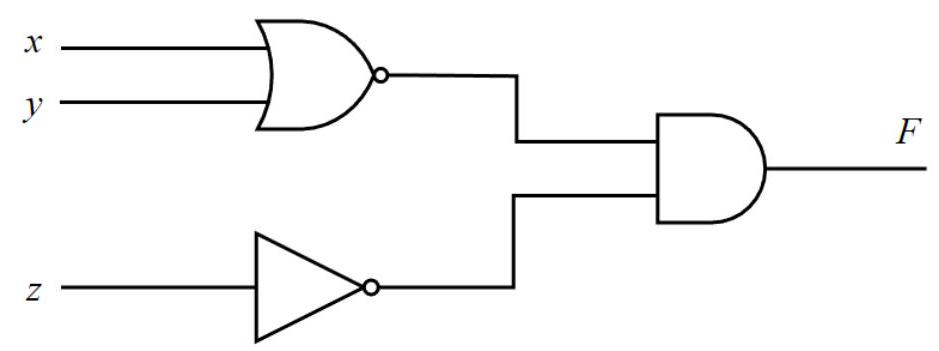
\includegraphics[max width=\textwidth]{2024_05_20_f1af48ad54173fe448ecg-2}
\end{center}

\section*{一、集成电路简介}
\section*{二、MOSFET 工作原理}
\begin{enumerate}
  \setcounter{enumi}{3}
  \item 请回答下列问题 2 :
\end{enumerate}

a) 请画出作为四端器件的 NMOS 和 PMOS 晶体管的电路符号, 并在图中标注出这些端口。

b) 请写出 MOSFET 的各工作模式以及对应的电压和电流关系。

c) 请解释速度饱和效应并简要分析其对晶体管工作的影响。

\section*{三、CMOS 反相器 VTC 特性分析}
\begin{enumerate}
  \setcounter{enumi}{4}
  \item 请画出一个反相器的 VTC 的大致形状, 并在图中标注出不同的工作状态。

  \item 对于噪声容限 (Noise Margin):

\end{enumerate}

a) 请解释噪声以及噪声容限的定义。

b) 给定一个反相器的 VTC 图, 如何得到其噪声容限?请举例说明。

\section*{四、CMOS 反相器延时与功耗分析}
\begin{enumerate}
  \setcounter{enumi}{6}
  \item 对于静态 CMOS 反相器:
\end{enumerate}

a) 请画出一个标准反相器的内部构造图, 并标注出晶体管的尺寸比例。

b) 请分析反相器的尺寸变化对电阻, 电容以及延时的影响。

\section*{五、静起 CMOS 㵋辑门设计与优化}
\begin{enumerate}
  \setcounter{enumi}{7}
  \item 请根据下述逻辑表达式回答问题:
\end{enumerate}

$$
\text { Out }=\overline{D+A(B+C)}
$$
\footnotetext{${ }^{2}$ 此类型题目的目的为知识回顾, please don't panic, 考试中不会出现复杂知识点以及公式的默写
}
a) 请设计完成能实现该逻辑功能的静态 $\mathrm{CMOS}$ 逻辑门。

b) 请写出逻辑门延时的计算方法 (不包括中间电容)。

c) 设负载电容为 $\boldsymbol{C}_{L}$, 标准反相器的输入电容和寄生电容分别为 $\boldsymbol{C}_{g, o}$ 和 $C_{p a r, 0}$, 请计算 a) 中得到的逻辑门的传播延时。

\begin{enumerate}
  \setcounter{enumi}{8}
  \item 对于一个 2 输入的异或 (XOR) 门, 请回答下列问题:
\end{enumerate}

a) 请写出它的真值表, 并使用 SOP (Sum Of Product) 的方法写出它的逻辑表达式。

b) 设负载电容为 $\boldsymbol{C}_{L}$, 标准反相器的输入电容和寄生电容分别为 $\boldsymbol{C}_{g, \boldsymbol{n}}$ 和 $C_{p a r, 0}$, 请计算它的传播延时。

c) 对于该门的两个输入 $\boldsymbol{A}$ 与 $\boldsymbol{B}$, 假设 $\boldsymbol{P}_{A=1}=1 / 3, P_{B=1}=1 / 2$, 请计算该门的切换功耗。

\begin{enumerate}
  \setcounter{enumi}{9}
  \item 对于一个 2 输入的同或(XNOR)门, 请回答下列问题:
\end{enumerate}

a) 请设计出能完成其功能的静态 CMOS 逻辑门。

b) 对于该门的两个输入 $\boldsymbol{A}$ 与 $\boldsymbol{B}$, 假设 $\boldsymbol{P}_{A=1}=1 / 3, P_{B=1}=1 / 2$, 请计算该门的切换功耗。

\begin{enumerate}
  \setcounter{enumi}{10}
  \item 请根据下列逻辑表达式回答问题:
\end{enumerate}

$$
\text { Out }=(A \bar{B}+C) D
$$

a) 请设计完成能实现该逻辑功能的静态 $\mathrm{CMOS}$ 逻辑门。

b) 请使用与 a)不同的方案实现同样具有逻辑功能的静态 CMOS 逻辑门。

\begin{enumerate}
  \setcounter{enumi}{11}
  \item 下图是一个 2 输入的同或 (XNOR) 门的符号表示, 请回答下列问题:
\end{enumerate}

\begin{center}
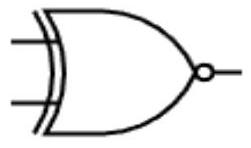
\includegraphics[max width=\textwidth]{2024_05_20_f1af48ad54173fe448ecg-3}
\end{center}

a) 请写出它的真值表以及逻辑表达式。

b) 请使用静态 CMOS 电路实现该逻辑门。

\begin{enumerate}
  \setcounter{enumi}{12}
  \item 对于多输入的异或 (XOR) 门该如何工作, 向来众说纷纭。有人将其称为 “奇数功能或门”, 即当奇数个输入为高电平时, 其输出为高电平。请回答下列问题:
\end{enumerate}

a) 请写出使用以上定义实现的 3 输入 XOR 门的真值表并设计出能实现其逻辑功能的静态 $\mathrm{CMOS}$ 电路。

b) 你认同这种定义吗? 你认为多输入的 XOR 门应该实现什么样的逻辑功能?

\begin{enumerate}
  \setcounter{enumi}{13}
  \item (数字逻辑相关)请回答下列问题:
\end{enumerate}

a) 什么是逻辑运算的最小完全集?\\
b) $\{$ 与,或,非 $\}$ 是一个最小完全集吗?\{与非,或非\}呢?

c) 请使用 NAND 门与 NOR 门实现 AND, OR 与 INV 门, 再使用 AND, OR 与 INV 门实现 NAND 门与 NOR 门 (2 输入)。

\begin{enumerate}
  \setcounter{enumi}{14}
  \item 请根据下述逻辑表达式回答问题:
\end{enumerate}

$$
\text { Out }=\overline{A B C+\bar{A} B+B \bar{C}+A C}
$$

a) 该表达式能否进一步化简?请写出化简后的表达式。

b) 根据原表达式或者 a) 中得到的结果, 实现对应的静态 CMOS 逻辑门。

\begin{enumerate}
  \setcounter{enumi}{15}
  \item 请结合以下真值表回答问题:
\end{enumerate}

\begin{center}
\begin{tabular}{|l|l|l|}
\hline
$\boldsymbol{A}$ & $\boldsymbol{B}$ & $\boldsymbol{Y}$ \\
\hline
0 & 0 & 0 \\
\hline
0 & 1 & 0 \\
\hline
1 & 0 & 1 \\
\hline
1 & 1 & 1 \\
\hline
\end{tabular}
\end{center}

a) 请根据真值表写出对应的逻辑表达式。

b)请根据逻辑表达式实现对应的静态 $\mathrm{CMOS}$ 电路。

\begin{enumerate}
  \setcounter{enumi}{16}
  \item 对于一个 4 输入的 NAND 门:
\end{enumerate}

a) 请写出其逻辑表达式。

b)使用互补 CMOS 设计将其实现,需要多少个 NMOS 晶体管?

\begin{enumerate}
  \setcounter{enumi}{17}
  \item 请解释静态 $\mathrm{CMOS}$ 电路中为什么使用 PMOS 晶体管实现 PUN 部分, 使用 NMOS 实现 PDN 部分? 若是互相替换会导致什么后果?

  \item 请结合下图回答问题:

\end{enumerate}

\begin{center}
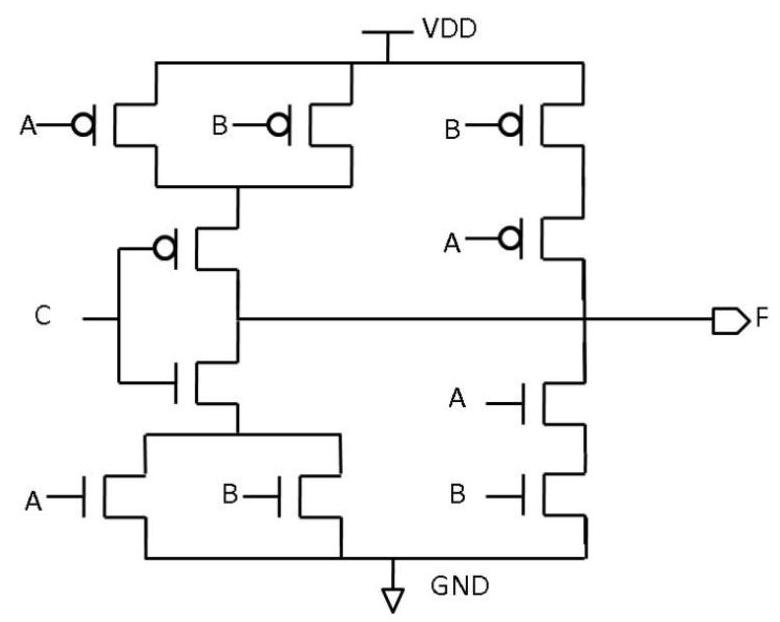
\includegraphics[max width=\textwidth]{2024_05_20_f1af48ad54173fe448ecg-5}
\end{center}

a) 图中的电路实现了什么样的逻辑功能?请写出其逻辑表达式。

b) 这是一个静态 CMOS 电路吗? 为什么?

\begin{enumerate}
  \setcounter{enumi}{19}
  \item 请结合下图回答问题:
\end{enumerate}

\begin{center}
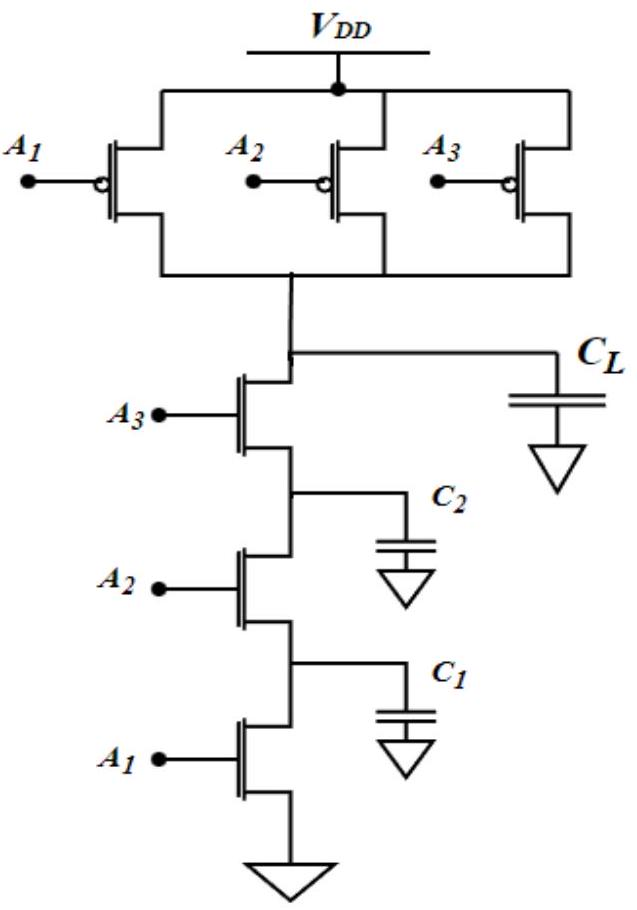
\includegraphics[max width=\textwidth]{2024_05_20_f1af48ad54173fe448ecg-5(1)}
\end{center}

a) 该图中的 CMOS 电路实现了什么样的逻辑功能? 请写出其逻辑表达式。

b) 假设该电路之前的状态为: $\boldsymbol{A}_{1}=0, \boldsymbol{A}_{2}=1, \boldsymbol{A}_{3}=1$, 请写出稳定时电路中几个电容的充放电状态。这时候如果 $\boldsymbol{A}_{1}$ 的状态由 0 变为 1 , 电容中的电荷会发生什么样的变化?

c) 结合 b) 中的情况, 如果输入中只有 $\boldsymbol{A}_{1}$ 会频繁地发生变化, 该电路的设计可能会导致什么问题? 能否进行优化?

\section*{六、Logical Efforts 分析方法介绍与应用}
\begin{enumerate}
  \setcounter{enumi}{20}
  \item (基础回顾)对于下图所示的静态 CMOS 逻辑门, 请回答:
\end{enumerate}

\begin{center}
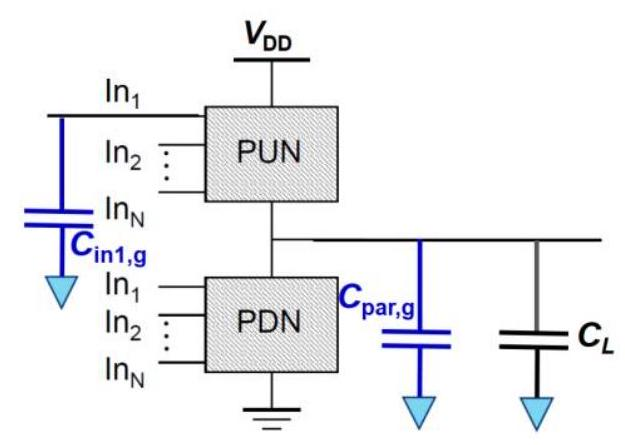
\includegraphics[max width=\textwidth]{2024_05_20_f1af48ad54173fe448ecg-6(1)}
\end{center}

a) 如何计算它的传播延时?请写出其传播延时的计算公式。

b) 图中的 $C_{i n l, g} 、 C_{p a r, g}, C_{L}$ 各代表了什么?

c) 如果将该门中所有晶体管的尺寸增大或缩小 $S$ 倍, 会对它的等效电阻和电容造成什么样的影响?

\begin{enumerate}
  \setcounter{enumi}{21}
  \item (Gate Sizing) 假设一个标准反相器的等效电阻为 $R_{I N V}, \operatorname{PMOS}$ 的 $W / L=2$, NMOS 的 $W / L=1$, 输入电容 (input capacitance) 为 $C_{i n, I N V}$, 寄生电容 (parasitic capacitance) 为 $C_{p a r: N N}$ 。同时假设负载电容为 $C_{L}$, 请回答下列问题:
\end{enumerate}

d) 对于一个 2 输入的 NAND 门, 请使用静态 CMOS 方法将其实现, 为其分配合适的尺寸使得其等效电阻等于 $R_{I N V}$, 并计算它的传播延时。

e) 对于一个 2 输入的 NOR 门, 请使用静态 CMOS 方法将其实现, 为其分配合适的尺寸使得其等效电阻等于 $R_{I N V}$, 并计算它的传播延时。

f) 对于一个 2 输入的 XOR 门, 请使用静态 CMOS 方法将其实现, 为其分配合适的尺寸使得其等效电阻等于 $R_{I N V}$, 并计算它的传播延时。

\begin{enumerate}
  \setcounter{enumi}{22}
  \item (Logical Effort) 下图是一个多级组合逻辑电路的示例, 请回答以下问题:
\end{enumerate}

\begin{center}
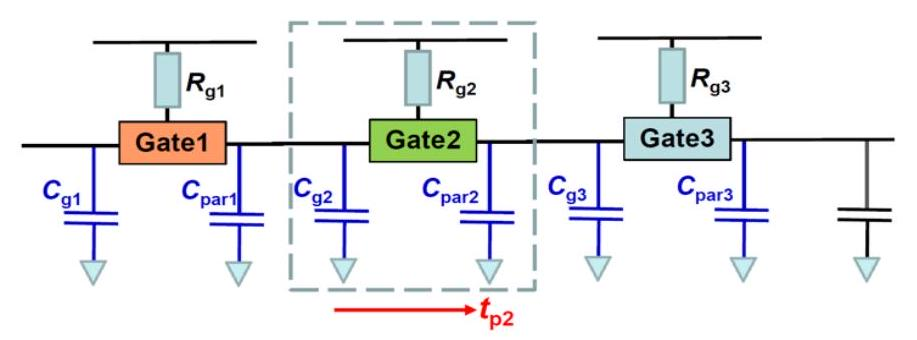
\includegraphics[max width=\textwidth]{2024_05_20_f1af48ad54173fe448ecg-6}
\end{center}

g) 如何计算多级组合逻辑电路的传播延时?请用自己的语言描述大致计算流程。

h) 如何使用 Logical Effort 方法计算多级组合逻辑电路的传播延时?请推导出其计算公式。

i) Logical Effort 方法中的电气扇出 $h$, 逻辑努力 $g$ 和本征延时 $p$ (Intrinsic

Delay/Parasitic Delay)代表了什么内涵?请写出它们的计算方法以及你对它们的理解。

j) 请补充下表的内容(计算逻辑努力 $g$ ):

\begin{center}
\begin{tabular}{|c|c|c|c|c|c|}
\hline
\multirow{2}{*}{类型} & \multicolumn{6}{|c|}{输入数量 $-\boldsymbol{g}$} \\
\cline { 2 - 6 }
 & 1 & 2 & 3 & 4 & $\mathrm{n}$ &  \\
\hline
NAND &  &  &  &  &  &  \\
\hline
NOR &  &  &  &  &  &  \\
\hline
MUX &  &  &  &  &  &  \\
\hline
XOR, XNOR &  &  &  &  &  &  \\
\hline
\end{tabular}
\end{center}

k) 请补充下表内容(计算本征延时 $p$ )

\begin{center}
\begin{tabular}{|c|c|}
\hline
类型 & Intrinsic Delay/Parasitic Delay $(p)$ \\
\hline
INV & 1 \\
\hline
n-input NAND &  \\
\hline
n-input NOR &  \\
\hline
n-way multiplexer &  \\
\hline
XOR, XNOR &  \\
\hline
\end{tabular}
\end{center}

\begin{enumerate}
  \setcounter{enumi}{23}
  \item (反相器链)设标准反相器的等效电阻为 $R_{I N V}$, 请计算出下图所示的反相器链的传播延时。
\end{enumerate}

$$
\text { Assume for unit width: } \begin{aligned}
& \mathrm{C}_{\mathrm{g}, 0}=1 \\
& \mathrm{C}_{\mathrm{par}, 0}=1
\end{aligned}
$$

\begin{center}
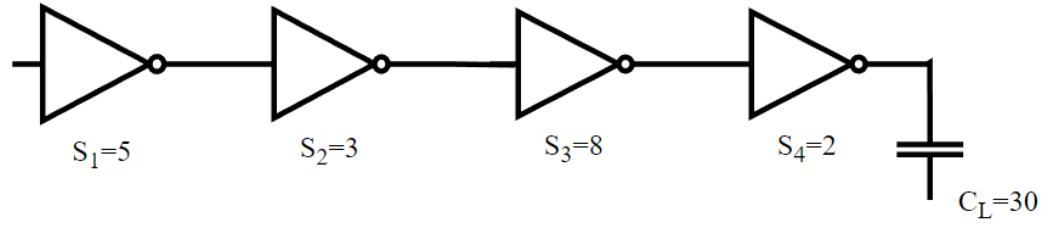
\includegraphics[max width=\textwidth]{2024_05_20_f1af48ad54173fe448ecg-7}
\end{center}

\begin{enumerate}
  \setcounter{enumi}{24}
  \item (传播延时) “提出问题往往比解决问题更重要”, 对于下图所示例题, 如果只给出所有门的 $W_{P}: W_{N}$, 能否计算出正确结果? 如果只给出 $\mathrm{S}$, 能否计算?如果只给出反相器的构造信息,能否计算?请根据图中的条件使用传统方法计算该电路的传播延时。
\end{enumerate}

\section*{Example: Delay of Multi-Stage Network}
\begin{center}
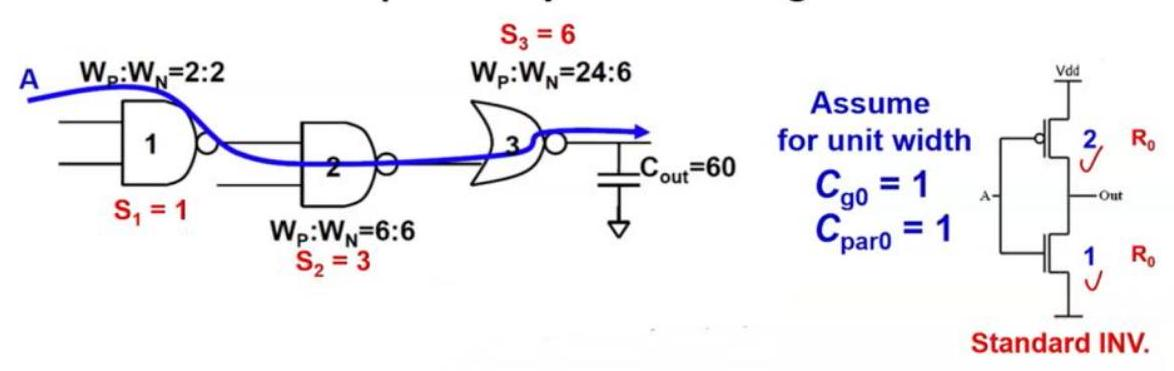
\includegraphics[max width=\textwidth]{2024_05_20_f1af48ad54173fe448ecg-8(1)}
\end{center}

\begin{enumerate}
  \setcounter{enumi}{25}
  \item 请使用逻辑努力(Logical effort)方法计算上图中的例题。

  \item 对于下图所示电路, 请计算出当传播延迟最小时, 每一级电路的晶体管尺寸大小 (假设对于单位宽度晶体管, $\mathrm{C}_{\mathrm{g}}=1, \mathrm{C}_{\mathrm{par}}=1$ )。

\end{enumerate}

\begin{center}
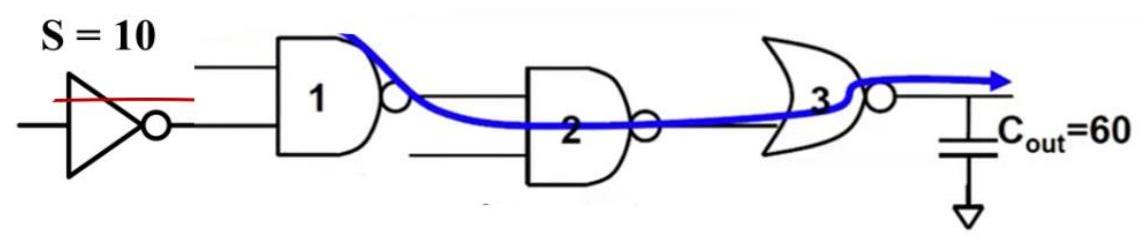
\includegraphics[max width=\textwidth]{2024_05_20_f1af48ad54173fe448ecg-8}
\end{center}


\end{document}